\documentclass{beamer}
 
\usepackage[USenglish]{babel}
\usepackage[T1]{fontenc}
\usepackage[utf8]{inputenc}
\usepackage{inputenc} 
\usepackage{graphicx}
\usepackage{float}
\usepackage{lmodern}
\usepackage{xcolor}
\usepackage{pifont}
\usepackage{amsmath}
\usepackage{booktabs}
%\usepackage[round]{natbib}
%\newcommand{\newblock}{}
%\usepackage{bibentry}
\usepackage{dsfont}
\usepackage{colortbl}
\usepackage{bm}
%\nobibliography*

 \usepackage{ragged2e}
\usepackage[
backend=bibtex,
style=alphabetic,
citestyle=authoryear,,maxbibnames=9,maxcitenames=2,
]{biblatex}

\usepackage{tikz,overpic}
\usetikzlibrary{fit,shapes.misc}

\usepackage{algorithm,algorithmic}

\graphicspath{{/home/administrateur/Documents/postdoc/cours_UCLA/figures/prmlfigs-pdf/}}

\definecolor{CustomBlue}{rgb}{0.2,1,1}

\setbeamercovered{transparent}

\footnotesize{
\bibliography{refs.bib}}
%\addbibresource{refs.bib}
\renewcommand*{\mkbibparens}[1]{{\ifcitation{\bibleftbracket#1\bibrightbracket}%
    {\bibleftparen#1\bibrightparen}}}
\renewcommand*{\bibopenparen}[1]{{\ifcitation{\bibleftbracket#1}{\bibleftparen#1}}}
\renewcommand*{\bibcloseparen}{{\ifcitation{\bibrightbracket}{\bibrightparen}}}

%\newcommand\footcite[1]{\footnote{\tiny{\bibentry{#1}\label{\thepage:#1}}}}
\newcommand\mycite[2][]{{\textcolor{blue}{\scriptsize\parencite[#1]{#2}}}}
\newcommand\myothercite[2][]{{\textcolor{cyan}{\scriptsize\parencite[#1]{#2}}}}
\newcommand\iamauthorcite[2][]{{\textcolor{magenta}{\scriptsize\parencite[#1]{#2}}}}
\usepackage{tikz}

\newcommand{\norm}[1]{\left\lVert#1\right\rVert}
\newcommand\given[1][]{\:#1\rvert}

\newcommand\numberthis{\addtocounter{equation}{1}\tag{\theequation}}

\usetheme{Warsaw}
%\useoutertheme[subsection=false]{smoothbars}

\newcommand{\cfbox}[2]{%
    \colorlet{currentcolor}{.}%
    {\color{#1}%
    \fbox{\color{currentcolor}#2}}%
}
%\setbeamertemplate{headline}{}

%\AtBeginSection[]
%{
%  \begin{frame}<beamer>
%    \addtocounter{framenumber}{-1}
%    \tableofcontents[currentsection]
%  \end{frame}
%}

\setbeamertemplate{footline}[frame number]{}
%\AtBeginSubsection[]
%{
%    \begin{frame}{Outline}
%    \addtocounter{framenumber}{-1}
%        \tableofcontents[currentsection,currentsubsection]
%    \end{frame}
%}


\title[]{\textcolor{white}{\normalsize{Data Science for Geoscience 2020}}}
\author{{Lucas Drumetz\\
lucas.drumetz@imt-atlantique.fr}}
\date{\small{Data Science for Geoscience 2020, Toulouse}\\
Introductory lecture: Statistics and probability, Data exploration}



\setbeamertemplate{headline}{}

\begin{document}

%gets rid of navigation symbols

\setbeamertemplate{navigation symbols}{}
\expandafter\def\expandafter\insertshorttitle\expandafter{%
  \insertshorttitle\hfill%
  \insertframenumber\,/\,\inserttotalframenumber}

\newcommand\blfootnote[1]{%
  \begingroup
  \renewcommand\thefootnote{}\footnote{#1}%
  \addtocounter{footnote}{-1}%
  \endgroup
}

%\defbeamertemplate{description item}{align left}{\insertdescriptionitem\hfill}
%\setbeamertemplate{description item}[align left]



\AtBeginSection[]
{
  \begin{frame}
  \addtocounter{framenumber}{-1}
  \frametitle{Outline}
  \normalsize
%  \tableofcontents[currentsection]
      \tableofcontents
    [
  currentsection,
  sectionstyle=show/show,
  subsectionstyle=show/show/show
    ]
  \end{frame}
}



 
\begin{frame}
\titlepage
\end{frame}


\section{Descriptive Statistics}

\begin{frame}{Datasets}

A dataset can be seen as a collection of $N$ realizations of a $D$-dimensional random variable
\begin{equation*}
\mathbf{X} \in \mathbb{R}^{D\times N}
\vspace{-0.2cm}
\end{equation*}

Examples:
\begin{itemize}
\item Collection of grades among a population of $N$ students
\item The $N$ pixels of an image (gray-level $D=1$ or color $D = 3$)
\item A time series of data (e.g. the average temperature at a given location over time, $N$ is the number of time samples)
\item A time series of images (here $D$ can be the number of pixels and $N$ the number of time samples)
\end{itemize}
\vspace{-0.2cm}
\begin{center}
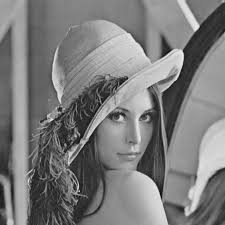
\includegraphics[scale=0.4]{lena.jpg} \hspace{0.2cm}
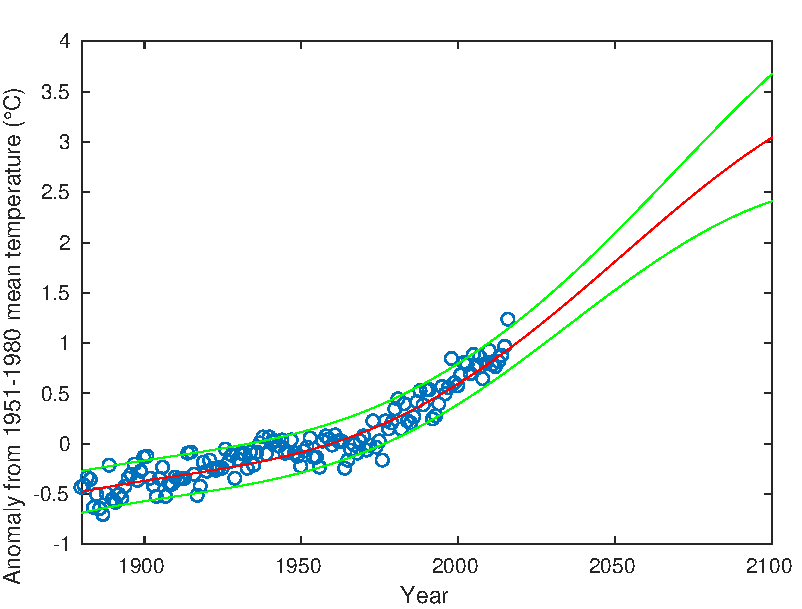
\includegraphics[scale=0.35]{gp_regression_nasa.pdf}

\end{center}

\end{frame}

\subsection{Univariate data}

\begin{frame}{Data description}



How can we describe univariate data (D=1) other than by a collection of values?\\

\begin{itemize}
\item Are certain values which are more probable than others?
\item Are the values centered on a particular value?
\item What is the spread around that value ?
\item Is the data symmetric around the central value?
\item Are there values that are very different from most others?
\end{itemize}

\vspace{0.25cm}
Ideally, we should know the probability density function (pdf)
\begin{equation*}
p(x)
\end{equation*}
$\rightarrow$ provides all the necessary information

\end{frame}

\begin{frame}{Descriptive Statistics}

\begin{itemize}
\item Estimate the pdf from the data
\item Compute quantities to try and answer the previous questions
\end{itemize}


\begin{block}{Statistical Independence}
Two random variables are independent if $p(x,y) = p(x)p(y)$
\end{block}

\begin{block}{Expected value of a (continuous) random variable}
\begin{equation*}
\mu = \mathbb{E}[x] = \int_{x \in \mathbb{R}} x p(x) \textrm{d}x
\end{equation*}

\end{block}

\begin{block}{Variance of a random variable}

\begin{equation*}
\sigma^2 = \textrm{Var}(x) = \mathbb{E}[(x-\mathbb{E}[x])^2] =  \mathbb{E}[x^2]-\mathbb{E}[x]^2
\end{equation*}
\end{block}

We also often use the standard deviation $\mathbf{\sigma} = \sqrt{\sigma^{2}}$

\end{frame}

\begin{frame}{Mean and variance estimation}
The expectation is approximated by the empirical mean

\begin{equation*}
\hat{\mu} = \frac{1}{N} \sum_{i=1}^{N} x_{i}
\end{equation*}


such that if the $x_{i}$ all follow the same distribution and are drawn independently:
\begin{align*}
& \mathbb{E}[\hat{\mu}] = \mu
& \textrm{Var}(\hat{\mu}) = \frac{\sigma^{2}}{N} \  \underset{N\rightarrow +\infty}{\longrightarrow} 0
\end{align*}

$\rightarrow$ The empirical mean is an estimator of the mean which is \emph{unbiaised} and \emph{consistent}\\

\vspace{0.5cm}

The variance of the data is approximated by the empirical variance:

\begin{equation*}
\hat{\sigma}^{2} = \frac{1}{N-1} \sum_{i=1}^{N} (x_{i} - \hat{\mu})^2
\end{equation*}

\end{frame}


\begin{frame}{Other statistical descriptors}
\begin{itemize}
\item Mode of the distribution: $\underset{x}{\textrm{arg\ max}} \ \ p(x)$
\item Median: value that separates the data into two subsets that are equiprobable\\
$\rightarrow$ empirical estimation:  value that splits the datasets into two subsets with the same number of samples\\
\vspace{0.5cm}

How is that different from the mean?\\
\vspace{0.2cm}
\raisebox{0.5\height}{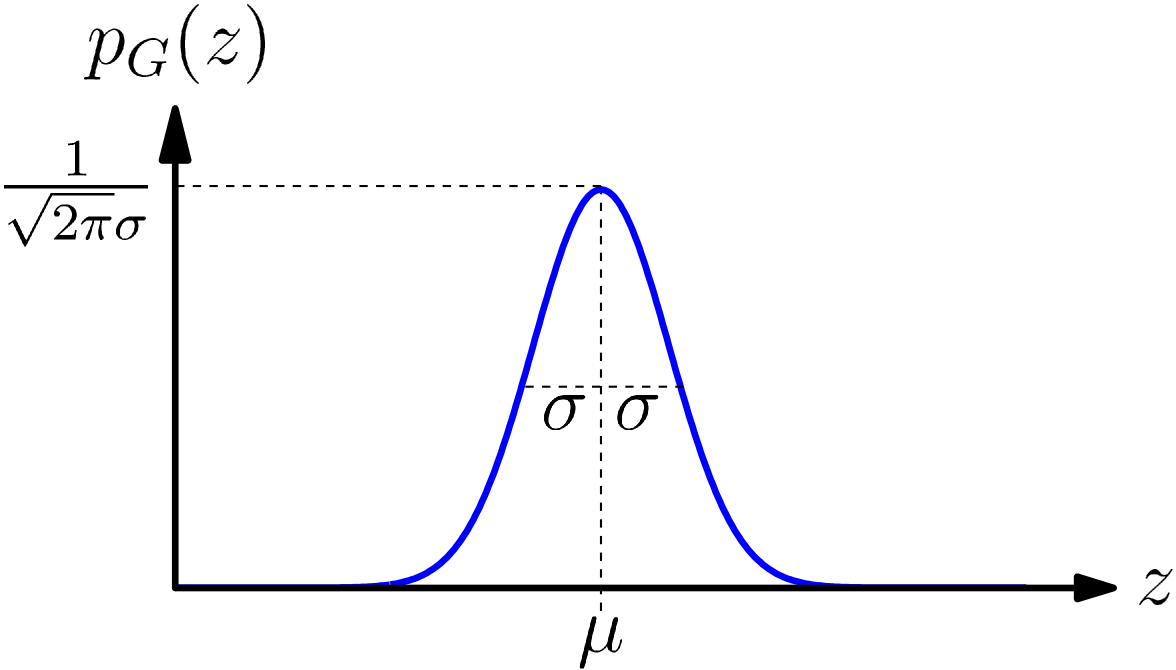
\includegraphics[scale=0.4]{gaussian.png}}
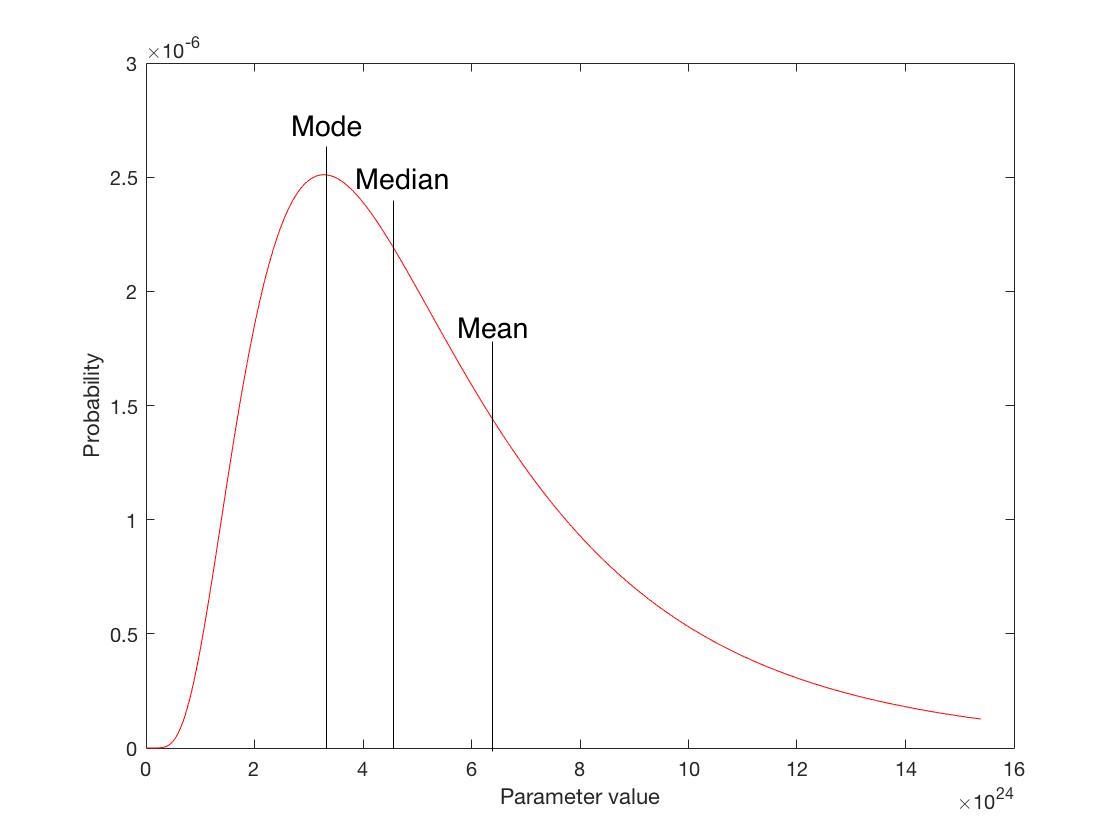
\includegraphics[scale=0.15]{modemeanmedian.jpg}

\end{itemize}
\end{frame}

\begin{frame}{Other statistical descriptors (cont'd)}

\begin{itemize}

\item Quantiles: generalization of the median\\
$\rightarrow$ the q-quantiles divide the domain into $q$ regions, all with probability $1/q$ (or $\textrm{floor}(N/q)$ samples)\\
\vspace{0.2cm}
Box plots use the median and the other quartiles (4-quantiles)
\begin{center}
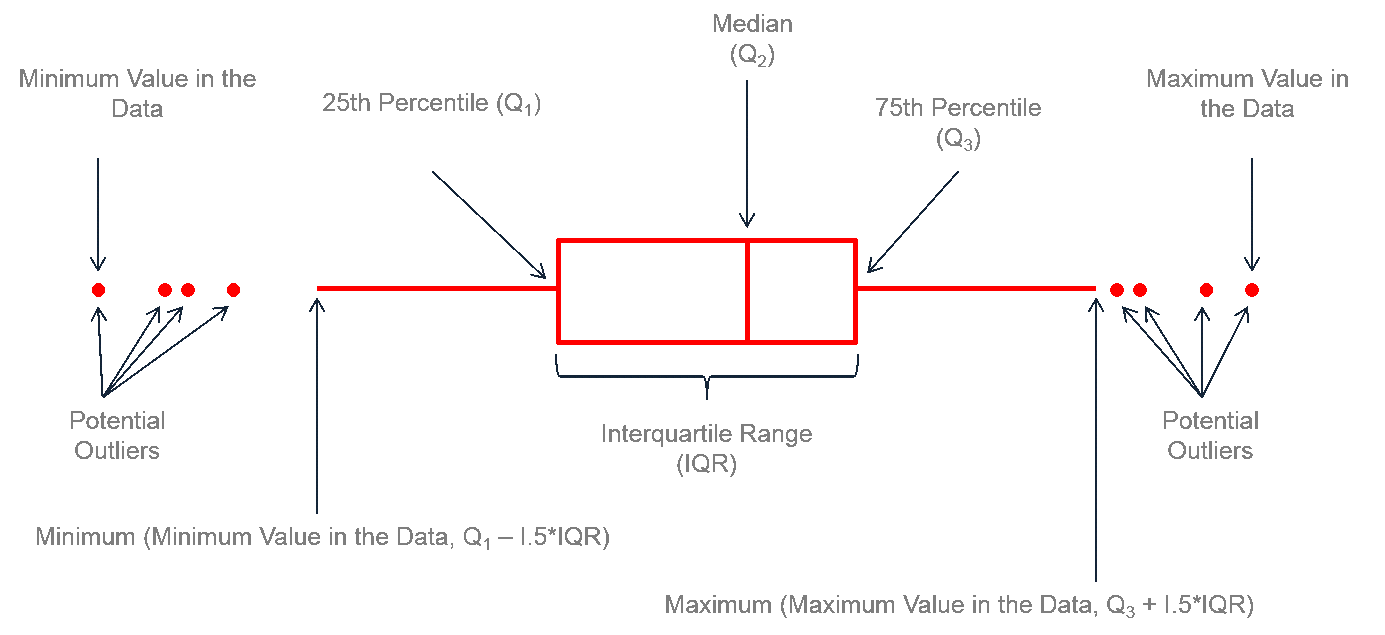
\includegraphics[scale=0.25]{boxplot_explanation.png}\\
\end{center}
\end{itemize}
\end{frame}


\begin{frame}{Other statistical descriptors (cont'd)}
\begin{itemize}
\item Higher order moments: related to $\mathbb{E}[x^{k}]$, $k > 2$\\
\begin{itemize}
\item 3rd order: Related to the assymetry of the distribution
\begin{block}{Skewness}
Skewness is a measure of symmetry of the distribution:
\begin{equation*}
\gamma = \mathbb{E}\left[ \left( \frac{x - \mu}{\sigma} \right) ^3 \right]
\end{equation*}
\begin{center}
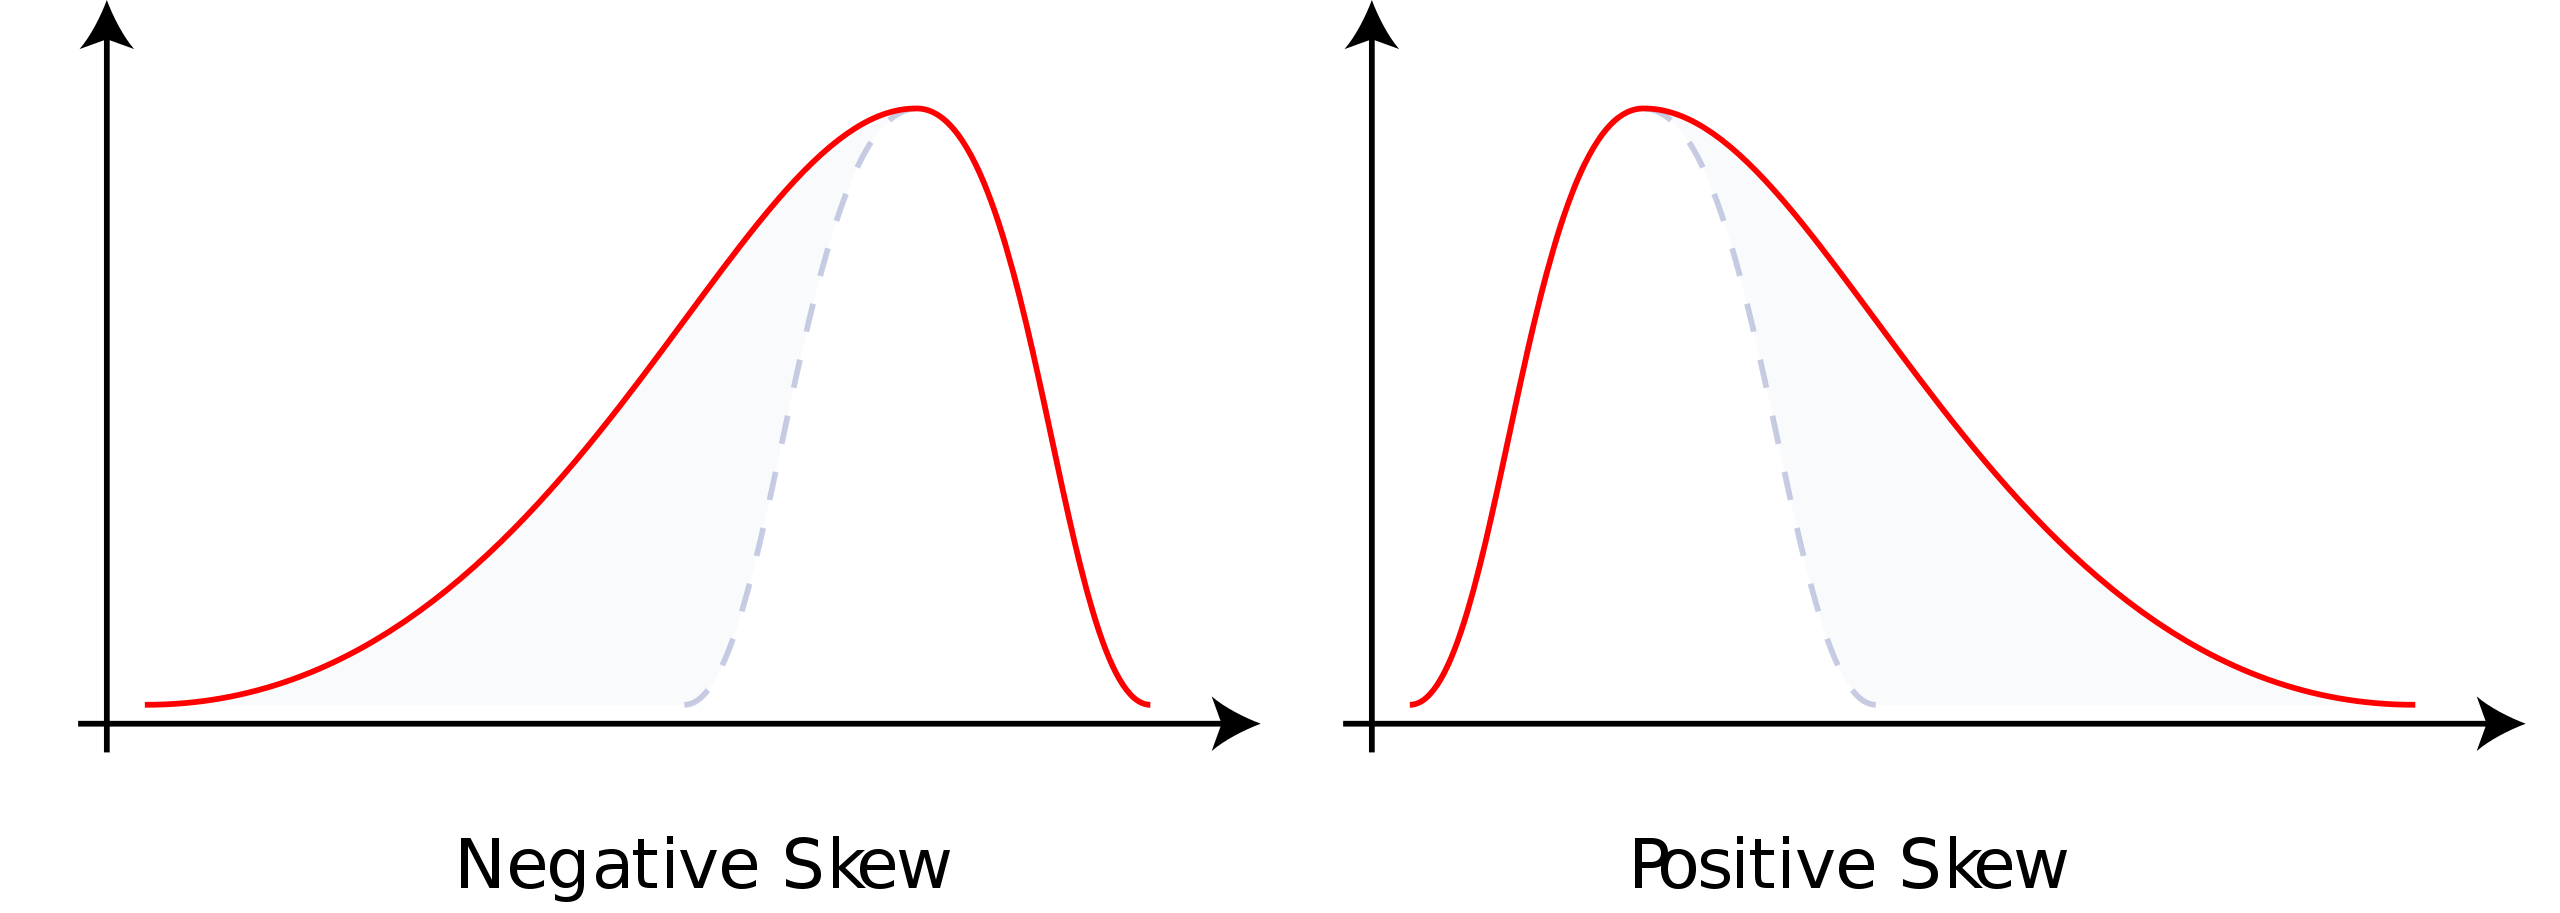
\includegraphics[scale=0.08]{skewness.png}\\
\tiny{$\gamma = 0$: symmetric distribution, $\gamma < 0$ (resp. $\gamma > 0$) distribution with a longer left tail (resp. right tail)}
\end{center}
\end{block}
\item 4th order: Quantifies how heavy the tails of the distribution are
\end{itemize} 

\end{itemize}
\end{frame}
\subsection{Multivariate data}

\begin{frame}{Multivariate data}
Multivariate data: D > 1, $\mathbf{x}_{i}$ is now a realization of a random vector.\\

\vspace{0.2cm}
Expectation:

\begin{equation*}
\mathbb{E}[\mathbf{x}] = \mathbb{E} \begin{bmatrix}
x_1\\
x_2\\
\vdots\\
x_D \end{bmatrix} =  \begin{bmatrix}
\mathbb{E}[x_1]\\
\mathbb{E}[x_2]\\
\vdots\\
\mathbb{E}[x_D] \end{bmatrix}
\end{equation*}



Notion of covariance:\\
\begin{equation*}
\textrm{Cov}(x_i,x_j) = \mathbb{E}[(x_i - \mathbb{E}[x_i])
(x_j - \mathbb{E}[x_j]) ] \in \mathbb{R}
\end{equation*}

Covariance matrix:\\

\begin{equation*}
\textrm{Cov}(\mathbf{x}) = \mathbb{E}[(\mathbf{x}- \mathbb{E}[\mathbf{x}])(\mathbf{x}- \mathbb{E}[\mathbf{x}])^{\top}] \in \mathbb{R}^{D\times D}
\end{equation*}

\end{frame}

\begin{frame}{Correlation and independence}

Two variables $X$ and $Y$ are uncorrelated if their covariance $\textrm{Cov}(X,Y)$ is zero
\\
\vspace{0.2cm}
Correlation is defined as 
\begin{equation*}
\textrm{Corr}(X,Y) = \frac{\textrm{Cov}(X,Y)}{\sigma_{X}\sigma_{Y}} \in [-1,1]
\end{equation*}
\begin{center}
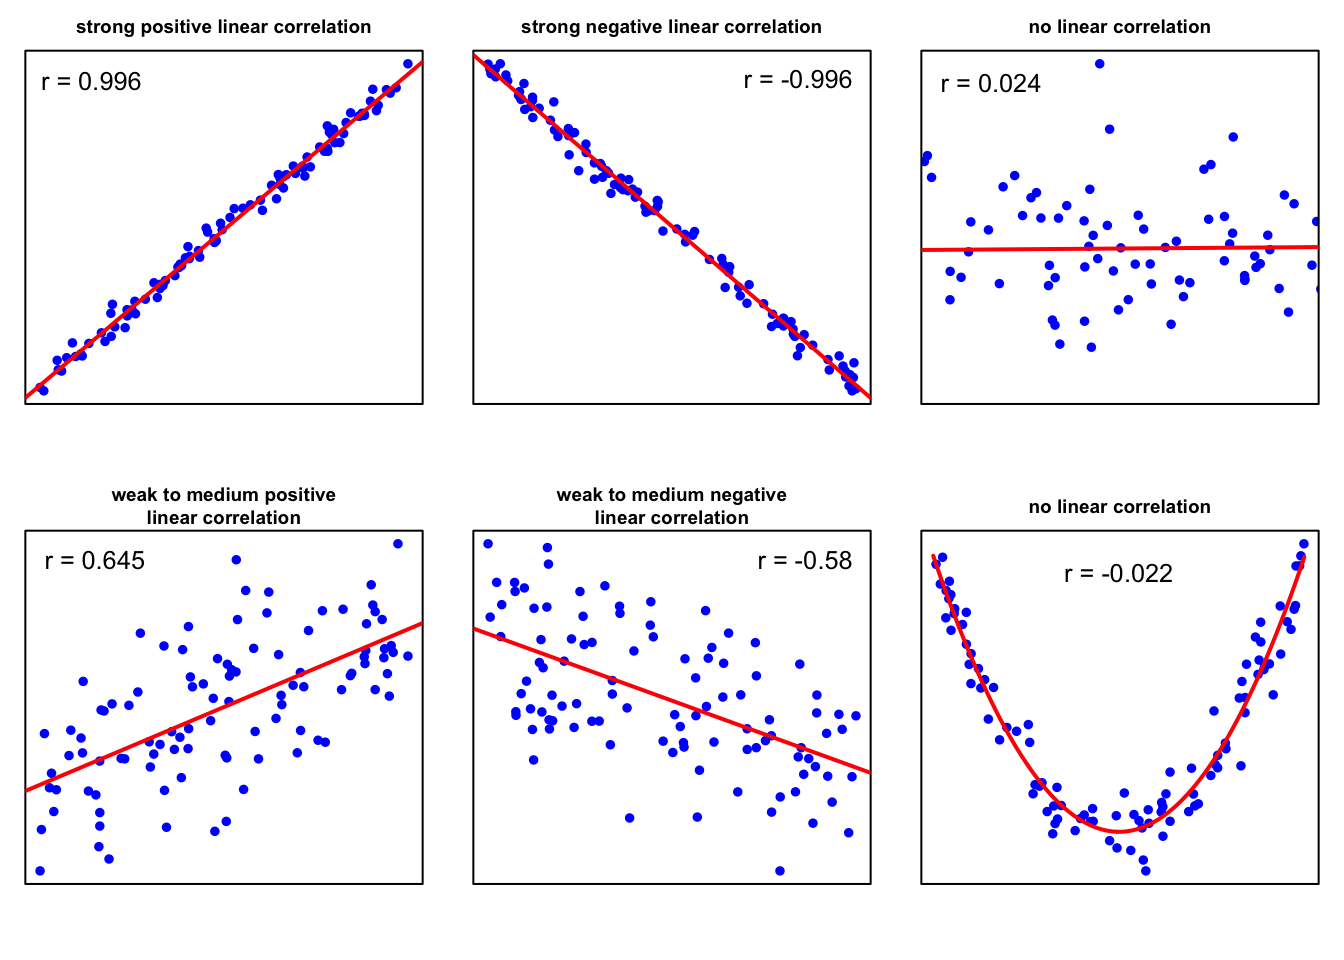
\includegraphics[scale=0.14]{correlation.png}
\end{center}
\vspace{-0.3cm}
Two uncorrelated variables can be dependent!\\ Example : $Y = X^2$, where $X$ is uniform on [-1,1].\\
\end{frame}

\begin{frame}{Correlation does not imply causation}
\begin{center}
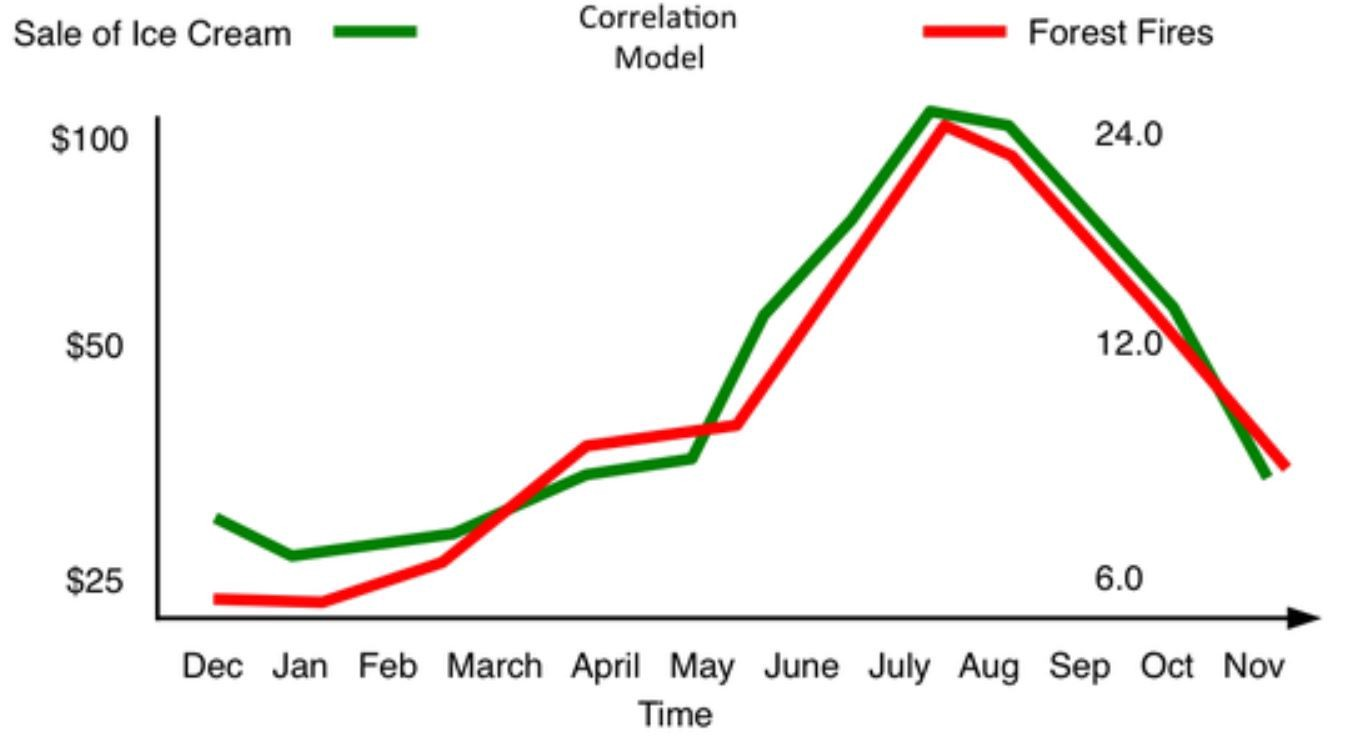
\includegraphics[scale=0.12]{correlation_causation.jpeg}\\
$\rightarrow$ In this case, both variables are caused by another common variable (i.e. the high temperatures in summer)\\
\vspace{0.4cm}
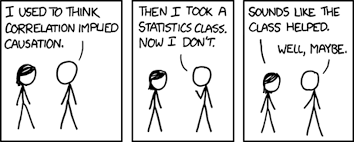
\includegraphics[scale=0.5]{correlation_causation_xkcd.png}\\
\end{center}
\end{frame}





\section{Outliers and Missing Values}
\subsection{Outliers}
\begin{frame}{Outliers}

There is no clear definition of what an outlier is, it is simply described as a data point which "significantly" differs from the rest.

\begin{block}{Possible causes}
\begin{itemize}
\item Data point which does not follow the same distribution as the others (e.g. measurement error)
\item The data has a heavy tailed distribution\\
\begin{center}
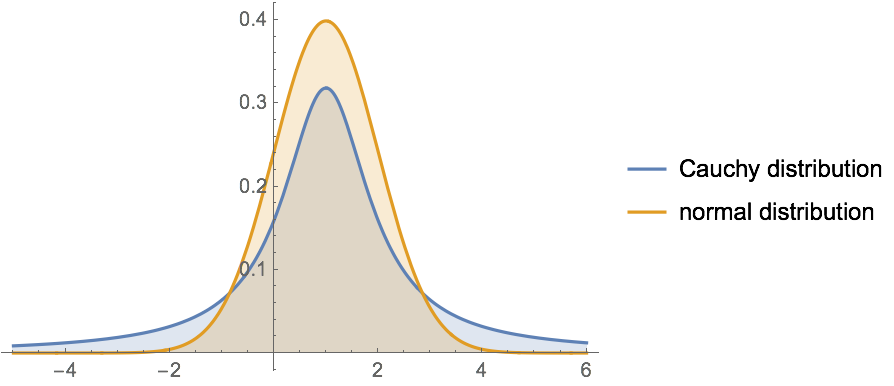
\includegraphics[scale=0.3]{NormalCaucy.png}
\end{center}
\end{itemize}
\end{block}

\end{frame}

\begin{frame}{Outliers}
\begin{block}{Examples of outliers in geoscience:}
\begin{itemize}
\item Optical images: sun glint saturating the sensor in a few pixels
\item Extreme values of geophysical fields (e.g. extreme wind gusts, rogue waves for sea surface heights...)
\item Sensor issues: dead pixels on a CCD device, numerical "salt and pepper" noise...
\end{itemize}
\end{block}


\begin{center}
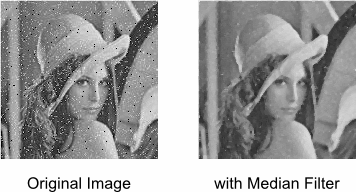
\includegraphics[scale=0.45]{midF.png}
\end{center}

\begin{itemize}
\item A possible strategy for outlier removal: Remove all data points such that $x \notin [median - 3\sigma, median + 3\sigma]$

Rationale: for the normal (Gaussian) distribution, a drawn sample has 99\% probability to be in this interval.
\end{itemize}

\end{frame}

\begin{frame}{Missing Values}
Missing values are frequent in geoscientific data. Ex:
\begin{itemize}
\item Cloud cover in optical imaging
\item "Along track" satellite acquisitions
\item Sensor issues
\item Boundaries: e.g. land pixels in oceanic variables
\end{itemize}

\begin{center}
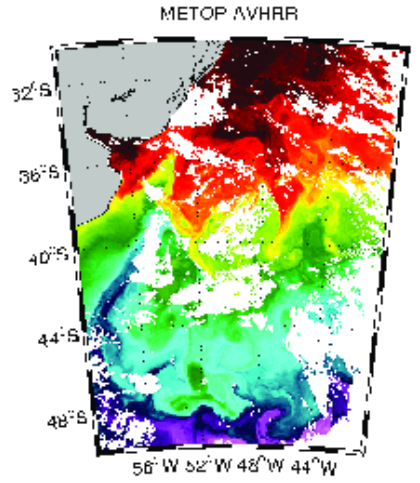
\includegraphics[scale=1.2]{sst_ex.png}
\raisebox{0.1\height}{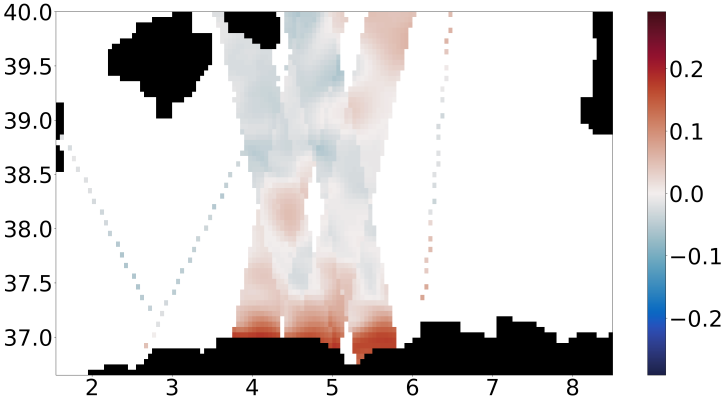
\includegraphics[scale=1.2]{ssh_ex.png}}\\
\tiny{Missing data in microwave Sea Surface Temperature (SST) data (left) and in altimetric Sea Surface Height (SSH) along track data (right)}
\end{center}

\end{frame}

\subsection{Missing Values}
\begin{frame}{Handling missing values}

There are different cases:

\begin{itemize}
\item The data points are just used in a statistical way (no use of the topology): then analyses can still be performed with a reduced number of points
\item The topology is used, and we need to fill in values: interpolation
\end{itemize}

\begin{block}{Interpolation}
\begin{itemize}
\item "Brutal" way: fill everything with zeros
\item Statistical way: try to combine and diffuse the information in observed points to unobserved ones
\item "Assimilation" way: Combine statistics and a priori physical information (a dynamical model for space time processes, coarse resolution auxiliary data...)
\end{itemize}
\end{block}

\end{frame}

\begin{frame}{Statistical interpolation techniques}


\begin{block}{Basic idea}
\begin{itemize}
\item Reconstruct the value of a desired grid point using a linear combination of all observations:
\vspace{-0.2cm}
\begin{equation*}
\mathbf{x} = \sum_{i=1}^{N} w_{i} \mathbf{d}_{i}
\end{equation*}
\item The weights can be calculated in several ways, and are typically higher for observed points close to the desired point and decay with the distance.
\end{itemize}
\end{block}

We define $r_{i} = ||\mathbf{d}_{i} -\mathbf{x}||_{2}$ for all grid points $\mathbf{x}$ and a parameter $R$.\\

Gaussian weights:
\begin{equation*}
\tilde{w}_{i} = \exp \left(\frac{-r_{i}^2}{2R^2}\right)
\end{equation*}

The weights are normalized so they sum to one over all the data:
\begin{equation*}
w_{i} = \frac{\tilde{w}_{i}}{\sum_{j=1}^{N} \tilde{w}_{j}}
\end{equation*}

\end{frame}

\begin{frame}{Optimal Interpolation}

\begin{block}{Idea}
Define a way to perform the interpolation which accounts for spatial/temporal correlations in a flexible way and that is statistically optimal under some hypotheses
\end{block}

State-space formulation: we define a state vector $\mathbf{x} \in \mathbb{R}^{P}$ containing all of our $P$ field values to estimate, and an observation vector $\mathbf{y} \in \mathbb{R}^{N}$ containing the values at the $N$ observed points.
\begin{align*}
&\mathbf{x} = \mathbf{x}_{b} + \boldsymbol{\eta} \\
&\mathbf{y} = \mathcal{H}(\mathbf{x}) +\boldsymbol{\epsilon}
\end{align*}

\begin{itemize}
\item $\mathbf{x}_{b}$ is a background estimation
\item $\boldsymbol{\eta}$ is the background error
\item $\mathcal{H}$ is an operator mapping the full state to the observations
\item $\boldsymbol{\epsilon}$ is the observation error
\end{itemize}

$\rightarrow$ OI finds the Best Linear Unbiaised Estimator (BLUE) of $\mathbf{x}$ given the uncertainties on the model and the observations.

\end{frame}

\section{Density Estimation}
\subsection{Parametric density estimation}

\begin{frame}{Probability density estimation}

Knowledge of $p(\mathbf{x})$ provides all the info on the variable\\
$\rightarrow$ Estimate it from data!\\

\vspace{0.2cm}

There are two ways of doing this:
\begin{itemize}
\item Assume the data follows a parametric density and estimate those parameters from data\\
$\rightarrow$ Maximum Likelihood estimation
\item Use non-parametric approaches to fit a pdf to the data\\
$\rightarrow$ Histograms and kernel density estimation
\end{itemize}



\end{frame}

\begin{frame}{Parametric density estimation}
\begin{itemize}
\item Assume that the data follows some distribution $p_{\boldsymbol{\theta}}(\mathbf{x})$ where $\boldsymbol{\theta}$ are the parameters of the distribution.
\item Find the values of the parameters $\boldsymbol{\theta}$ such that their value makes $p_{\boldsymbol{\theta}}(\mathbf{x})$ maximal:\\
\begin{equation*}
\hat{\boldsymbol{\theta}} = \underset{\boldsymbol{\theta}}{\textrm{arg max}} \ p_{\boldsymbol{\theta}}(\mathbf{x})
\end{equation*}

This procedure is called \emph{Maximum Likelihood} estimation

\item

In many cases, we have assume that the samples $\mathbf{x}_{i}$ are independent and identically distributed (i.i.d.), so that\\

\begin{equation*}
p_{\boldsymbol{\theta}}(\mathbf{X}) = \prod_{i=1}^{N}  p_{\boldsymbol{\theta}}(\mathbf{x}_{i})
\end{equation*}

\item Main advantage:the distribution is summarized by a small number of parameters

\end{itemize}
\end{frame}

\begin{frame}{Parametric density estimation (cont'd)}
\begin{block}{Example of the Gaussian}
\begin{itemize}
\item Assume that $\mathbf{x}_{i} \sim \mathcal{N}(\boldsymbol{\mu},\boldsymbol{\Sigma}) \ \forall i = 1,...,N$. Here $\boldsymbol{\theta}= (\boldsymbol{\mu},\boldsymbol{\Sigma}) $ (the pdf is completely specified by those two parameters) and \begin{equation*}
p_{\boldsymbol{\theta}}(\mathbf{x}) = \frac{1}{(2\pi)^{D/2} |\boldsymbol{\Sigma}|^{1/2}} \textrm{exp}\left(-\frac{1}{2} (\mathbf{x}-\boldsymbol{\mu})^{\top} \boldsymbol{\Sigma}^{-1} (\mathbf{x}-\boldsymbol{\mu}) \right)
\end{equation*}
\item Then, we can show that
\begin{equation*}
\hat{\boldsymbol{\mu}}_{ML}
 = \frac{1}{N} \sum_{i=1}^{N} \mathbf{x}_{i} \ \textrm{and} \
\hat{\boldsymbol{\Sigma}}_{ML} = \frac{1}{N} \sum_{i=1}^{N} (\mathbf{x} - \hat{\boldsymbol{\mu}})(\mathbf{x} - \hat{\boldsymbol{\mu}})^{\top}
\end{equation*}

\end{itemize}

\end{block}

Issues with parametric density estimation:\\
\begin{itemize}
\item Assumptions on the distribution are not always realistic
\item Estimation of the parameters can be cumbersome
\end{itemize}

\end{frame}

\subsection{Non Parametric density estimation}

\begin{frame}{Non-parametric density estimation}

\begin{block}{Histograms}
Divide the domain into bins of width $\Delta_{i}$ and count the number of occurrences $n_{i}$ of the data values in each bin.\\
\vspace{0.2cm}
Then we say that the probability that a data point falls into bin $\#i$ is given by
\begin{equation*}
p_{i} = \frac{n_{i}}{N \Delta_{i}}
\end{equation*}

This assumes that the pdf is piecewise constant
\\
\begin{center}
\includegraphics[scale=0.6]{Figure2_1.pdf}
\end{center}
\vspace{-0.6cm}
We can show that the $p_i$ define a valid pdf.
\end{block}

\end{frame}

\begin{frame}{Histograms (cont'd)}

The number of bins (or equivalently their width if it is the same for each bin) has to be tuned carefully.

\begin{center}
\includegraphics[scale=1]{Figure2_24.pdf}\\
\tiny{Histograms for density estimation. 50 points from the true (green) distribution have been sampled, and the pdf is approximated by histograms with different bin widths.}
\end{center}
\end{frame}

\begin{frame}{Kernel density estimation}
Consider a possible value of a vector RV $\mathbf{x}$, and a small region $\mathcal{R}$ such that $\mathbf{x}\in{\mathcal{R}}$. Then the probability mass of $\mathcal{R}$ is:
\begin{equation*}
P = \int_{\mathcal{R}} p(\mathbf{x})d\mathbf{x}
\end{equation*}

We observe $N$ realizations of the data. $P\in\mathcal{R}$ with probability $P$. Then, the probability that there are $K$ observations in $\mathcal{R}$ out of $N$ data points follows a binomial distribution $\textrm{Bin}(K|N,P)$.

\begin{equation*}
\mathbb{E}[K/N] = P, \ \textrm{and} \ \textrm{var}(K/N) = P(1-P)/N \underset{N\rightarrow \infty}{\rightarrow} 0
\end{equation*}

So, for large $N$, $K\approx NP$.\\
\end{frame}

\begin{frame}{Kernel Density Estimation}
In addition, if region $\mathcal{R}$ is small, $p(\mathbf{x})$ is almost constant on the support of the region (volume $V$):
\begin{equation*}
P \approx p(\mathbf{x})V
\end{equation*}

Finally:

\begin{equation*}
p(\mathbf{x}) \approx \frac{K}{NV}
\end{equation*}

Our goal is to estimate $p(\mathbf{x})$

\begin{itemize}
\item Choose $K$ and try to estimate $V$ locally:\\ \textbf{$K$-nearest neighbor approach}
\item Choose $V$ and try to estimate $K$:\\ \textbf{kernel density estimator}
\end{itemize}
\end{frame}

\begin{frame}{Kernel density estimator}

Let's choose the region $\mathcal{R}$ to be a small hypercube centered at $\mathbf{x}\in \mathbb{R}^{D}$.
We define the \emph{indicator function} (an example of kernel) of a hypercube centered on the origin and of "radius" $\frac{1}{2}$:
\begin{equation*}
k(\mathbf{u}) = \begin{cases}
    1& \text{if } |u_{i}|\leq 1/2, \ \forall i=1,...,D\\
    0             & \text{otherwise}
\end{cases}
\end{equation*}

Then $k(\frac{\mathbf{x}-\mathbf{x}_{n}}{h})$ is the indicator function of a hypercube centered at $\mathbf{x}$ of side $h$.
\begin{equation*}
K = \sum_{n=1}^{N} k\left(\frac{\mathbf{x}-\mathbf{x}_{n}}{h}\right)
\end{equation*}

And finally:
\begin{equation*}
p(\mathbf{x}) \approx \frac{K}{NV} = \frac{1}{N}\sum_{n=1}^{N} \frac{1}{h^{D}} k\left(\frac{\mathbf{x}-\mathbf{x}_{n}}{h}\right)
\end{equation*}

Note: This generalizes the framework of histograms!

\end{frame}

\begin{frame}{Kernel density estimator}


Trick: changing the function $k$ into a smoother one, e.g. a Gaussian of variance $h^{2}$ for each dimension (diagonal covariance matrix) :
\vspace{-0.3cm}
\begin{equation*}
p(\mathbf{x}) \approx \frac{K}{NV} = \frac{1}{N}\sum_{n=1}^{N} \frac{1}{(2\pi h^{2})^{D/2}} \exp\left(-\frac{||\mathbf{x}-\mathbf{x}_{n}||^{2}}{2h^2}\right)
\end{equation*}

Any function satisfying the axioms of a pdf can be chosen:
$k(\mathbf{u}) \geq 0 \  \textrm{and} \int k(\mathbf{u}) d\mathbf{u} = 1$


\begin{center}
\vspace{-0.2cm}
\includegraphics[scale=0.7]{Figure2_25.pdf}\\
\tiny{Gaussian Kernel density estimator on the same data as before}
\end{center}

Note: KDE can also be seen as an interpolation technique!
\end{frame}

\section{The Curse of Dimensionality}
\subsection{Working in High dimensions}

\begin{frame}{Problems in High Dimensions}

\begin{itemize}
\item Computing histograms in large dimensions is tricky because it requires to grid the domain\\
$\rightarrow$ The number of needed hypercubes to grid $[0,1]^{D}$ scales exponentially with the dimension $D$ of the data!\\
\begin{center}
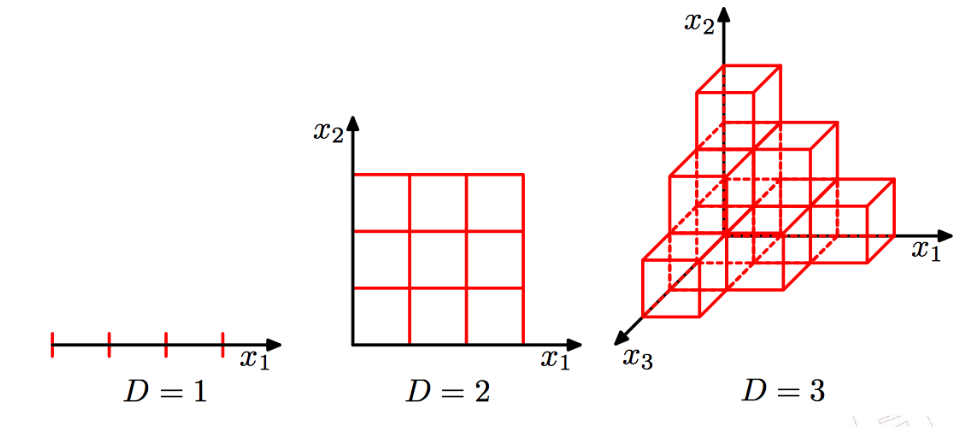
\includegraphics[scale=1]{hypercubes.png}
\end{center}
The volume of a single hypercube ($h^D$, $h<1$) also becomes smaller and smaller...\\
This means that data points are \emph{isolated} in a high dimensional space: you need exponentially more points for an "equivalent" sampling


\end{itemize}

\end{frame}

\begin{frame}{The curse of dimensionality}
\begin{itemize}
\item Visualizing data or probability distributions in more than 2-3D is hard
\item Parametric estimation also has issues: e.g. for a multivariate Gaussian, the number of parameters scales as $D^2$ (full covariance matrix): need to 
\begin{itemize}
\item estimate them from data (requires a large number of samples)
\item invert or find the eigenvalues of those matrices... (computing time scales in $\mathcal{O}(D^3)$)
\end{itemize}

\end{itemize}
\end{frame}

\begin{frame}{The curse of dimensionality (cont'd)}
The performance of learning tasks increases with the dimension of the features (more info) but only \emph{up to a point}\\
\vspace{0.2cm}
In high dimensions, the Euclidean distance does not separate data points well enough anymore

\begin{center}
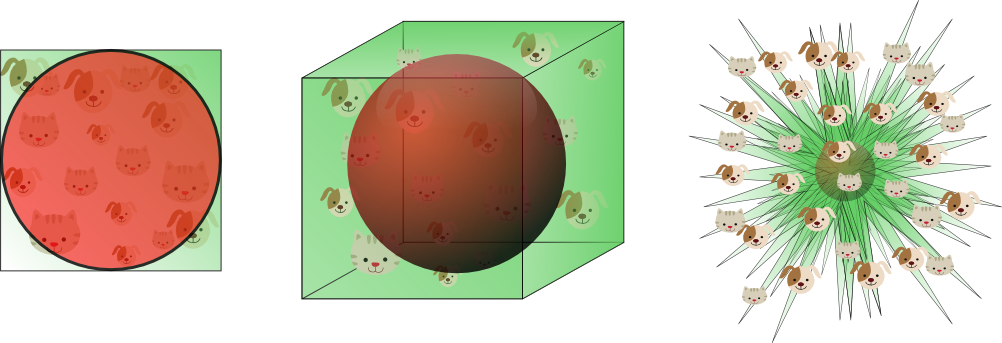
\includegraphics[scale=0.25]{ratio_volume.png}
\end{center}
\begin{equation*}
\frac{\textrm{Vol}_{Sphere}(D)}{\textrm{Vol}_{Cube}(D)}  \underset{D\rightarrow \infty}{\rightarrow 0}
\end{equation*}
This means that randomly sampled data points get further and further away from the mean and from eachother as $D$ grows. Every point is an outlier!
\end{frame}

\subsection{Visualizing High dimensional data}
\begin{frame}{Visualizing High dimensional data}
\begin{center}
\includegraphics[scale=0.725]{Figure12_1.pdf}\\
\tiny{Several transformed instances of the same "3" in the MNIST Digit dataset} ($100\times100$ images).
\end{center}

What is the actual dimensionality of the data?\\
$\rightarrow$ Each image can be seen as a point in $\mathbb{R}^{10^{4}}$\\
\vspace{0.5cm}
What is the number of degrees of freedom in all these data?\\
\begin{itemize}
\item Two Translations
\item One rotation
\item (With real instances of "3" images, several additional degrees from the variability of the writing of "3")
\end{itemize}
What is the \emph{intrinsic dimensionality} of the data?\\
%$\rightarrow$ Only 3 (or more in the real case), but the locus of the data is not a linear subspace

\end{frame}

\begin{frame}{Visualizing rotated images in 3D}
Only one degree of freedom here (one rotation).\\
Data still lives in $\mathbb{R}^{10^{4}}$. How can we visualize the feature space?
\begin{center}
\vspace{-0.4cm}
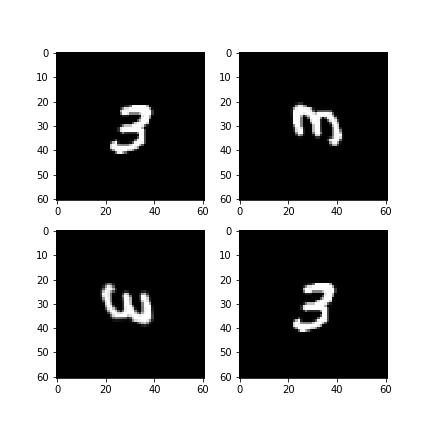
\includegraphics[scale=0.2]{rotated_3s.png}\\
\vspace{-0.35cm}
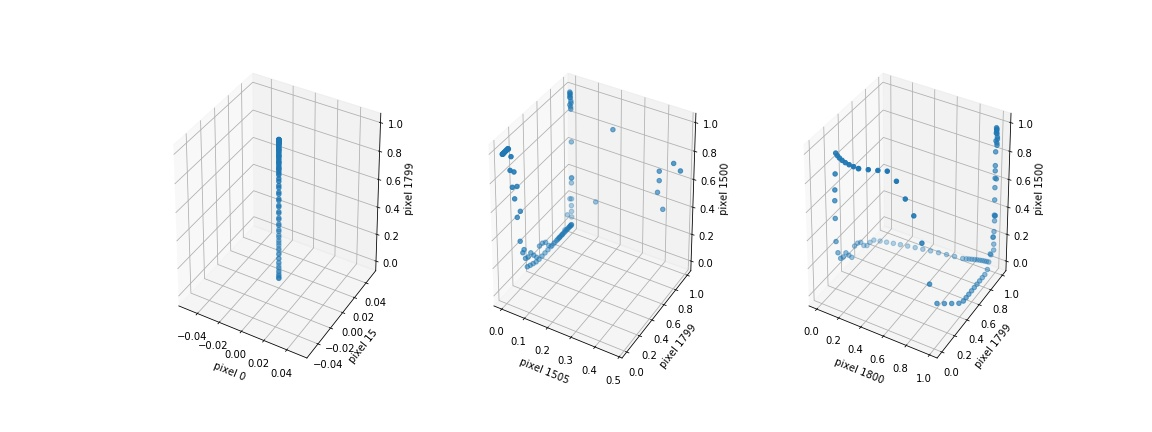
\includegraphics[scale=0.25]{scatterplots.jpg}\\
\end{center}
\vspace{-0.5cm}
$\rightarrow$ We need a way to summarize the information in only a few variables to visualize the data efficiently
\end{frame}

\section{Principal Component Analysis}


\subsection{Motivation}


%\footnotesize \let\small\footnotesize
\begin{frame}{Motivation}
High Dimensional datasets are often intrisically \emph{low-dimensional}.\\

$\rightarrow$ much fewer degrees of freedom than the dimensionality of the data.\\
\vspace{0.25cm}
This means that fewer variables than $D$ can summarize the information efficiently \\
\vspace{0.25cm}
The goal is to be able to recover \emph{latent variables} from the data.\\
\vspace{.25cm}
Applications:

\begin{itemize}
\item Dimensionality Reduction
\item Data compression
\item Data visualization
\item Feature Extraction
\item Denoising
\end{itemize}

%Typical latent variable model:
%
%%Example: linear Latent Variable model\\
%\begin{equation*}
%\mathbf{X} = \mathbf{SA}
%\end{equation*}
%
%$\mathbf{X}\in\mathbb{R}^{D\times N}$: data\\
%$\mathbf{S}\in\mathbb{R}^{D\times P}$ and $\mathbf{A}\in \mathbb{R}^{P\times N}$: latent variables
%
%$\mathbf{A}$ encodes a coefficient matrix\\
%$\mathbf{S}$ is a linear transformation\\


\end{frame}
\subsection{Algorithm}



\begin{frame}{Principal Component Analysis}

Basic idea: try to find a $P$-dimensional linear subspace which best represents the data in some sense.\\
\vspace{0.2cm}

%Chosen criteria: Find the subspace such that
%\begin{itemize}
%\item  the orthogonal projection of the data on it maximizes the variance of the projected data
%\item  the mean squared error between data points and their approximations using the orthogonal projections on the subspace is minimized
%\end{itemize}

Chosen criterion: Find the subspace such that the the variance of the orthogonal projection of the data on it is maximal


\begin{center}
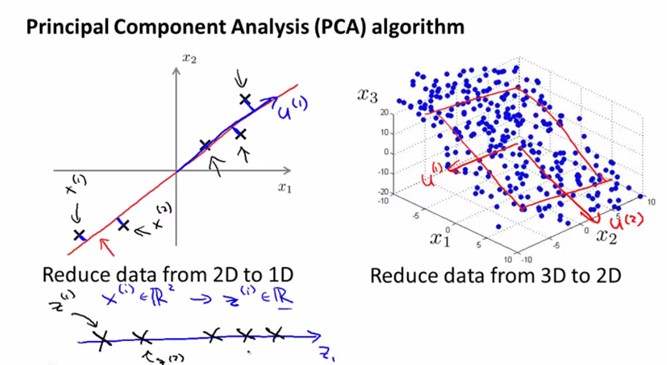
\includegraphics[scale=0.37]{pca_ex.jpg}
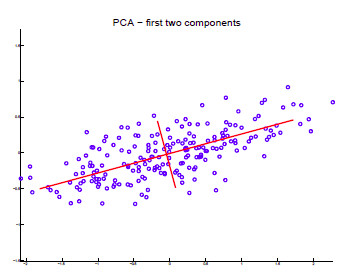
\includegraphics[scale=1.3]{pca_ex_1.jpg}\\
\end{center}
\vspace{-0.2cm}
Alternative criterion: find an orthogonal projection of the data on a subspace such that the projection error is minimal\\
\vspace{0.2cm}
$\rightarrow$ both formulations lead to the same solution and algorithm, called \emph{Principal Component Analysis}.

\end{frame}

%\begin{frame}{Lagrange Multipliers}
%
%Preliminary recap on Lagrange Multipliers:\\
%\vspace{0.25cm}
%Find stationary points of a real valued function of several variables subject to some constraints (only equality here):
%
%\begin{align*}
%& \underset{\mathbf{x} \in \mathbb{R}^{D}}{\textrm{arg max}} \ \  \ f(\mathbf{x}) \\
%& \textrm{s.t.} \quad \ \ \ \ \ \ g(\mathbf{x}) = 0
%\end{align*}
%
%\begin{center}
%\includegraphics[scale=0.2]{LagrangeMultipliers3D.png}\\
%\tiny{Minimize function $f$ (contour lines in blue) such that the solution lies on the red curve ($g(x^*,y^*)=0$).\\
%(source: Wikipedia)}
%\end{center}
%
%
%\end{frame}
%
%\begin{frame}{Lagrange Multipliers (cont'd)}
%\begin{itemize}
%\item For any point $\mathbf{x}$ on the constraint surface, $\nabla g(\mathbf{x})$ is orthogonal to the surface at this point.
%\item If $\mathbf{x}^{*}$ is optimal (i.e. on the constraint surface and minimizing $f$ subject to this constraint), then we also have $\nabla f(\mathbf{x}^*)$ orthogonal to the constraint surface.
%\end{itemize}
%
%Then $\nabla g(\mathbf{x}^*)$ and $\nabla f(\mathbf{x}^*)$ are parallel and we need to find a point such that:
%
%\begin{equation*}
%\nabla f(\mathbf{x}^*)+ \lambda \nabla g(\mathbf{x}^*) = 0
%\end{equation*}
%
%for some value of $\lambda \neq 0$ (called \emph{Lagrange Multiplier})\\
%\vspace{0.25cm}
%This amounts to nulling the gradient of the \emph{Lagrangian}:
%
%\begin{equation*}
%L(\mathbf{x},\lambda) = f(\mathbf{x}) + \lambda g(\mathbf{x})
%\end{equation*}
%
%The derivative w.r.t. $\lambda$ gives the constraint equation $g(\mathbf{x}) = 0$
%
%\end{frame}

\begin{frame}{Maximum Variance Formulation}

Goal: Define an \emph{orthogonal projection of the data} on a $M$-dimensional subspace, such that:
\begin{itemize}
\item the \emph{variance} of the data on the first component is maximal
\item the variance of the residual on the second component (orthogonal to the first) is maximal
\item and so on.
\end{itemize}

How to derive the first component?
$\rightarrow$ projection of the data on a line, directed by $\mathbf{u}_{1}$ (we choose $||\mathbf{u}_{1}||_{2}^{2}=\mathbf{u}_{1}^{\top}\mathbf{u}_{1}=1$)\\

\vspace{0.25cm}

The projection of a data point $\mathbf{x}_{n}$ on the line is:
\begin{equation*}
p(\mathbf{x}_{n}) = (\mathbf{u}_{1}^{\top}\mathbf{x}_{n})\mathbf{u}_{1}
\end{equation*}
The sample covariance of the \emph{projected} data is:
\begin{equation*}
\frac{1}{N} \sum_{n=1}^{N} (\mathbf{u}_{1}^{\top}\mathbf{x}_{n} -  \mathbf{u}_{1}^{\top} \bar{\mathbf{x}})^{2} = \mathbf{u}_{1}^{\top} \mathbf{S}\mathbf{u}_{1}
\end{equation*}

with $\bar{\mathbf{x}}$ is the sample mean of the data, and $\mathbf{S}$ its sample covariance.

\end{frame}

\begin{frame}{PCA: practical algorithm}
Now we need to solve:
\begin{align*}
& \textrm{arg max} \ \  \mathbf{u}_{1}^{\top}\mathbf{S}\mathbf{u}_{1}\\
& \textrm{s.t.} \ \quad ||\mathbf{u}_{1}||_{2}^{2} = 1
\end{align*}
The constraint removes degenerate solutions $||\mathbf{u}_{1}|| \rightarrow \ +\infty$\\
\vspace{0.2cm}

From this, we can show that there exists $\lambda_{1}$ such that the solutions verify
\begin{equation*}
\mathbf{S}\mathbf{u}_{1} = \lambda_{1} \mathbf{u}_{1}
\end{equation*}

There are several possibilities (one for each eigenvector of $\mathbf{S}$, symmetric and positive semidefinite matrix) and the corresponding variance is equal to:
\begin{equation*}
\mathbf{u}_{1}^{\top}\mathbf{S}\mathbf{u}_{1} = \lambda_{1}
\end{equation*}

$\rightarrow$  the one maximizing the variance is the eigenvector associated to the \emph{largest} eigenvalue.

\end{frame}

\begin{frame}{\textcolor{white}{Optimization for Maximum Variance}}

To obtain the remaining components, we simply have to repeat the process on the residual data:
\begin{equation*}
\hat{\mathbf{x}}_{n} = \mathbf{x} - (\mathbf{u}_{1}^{\top}\mathbf{x}_{n})\mathbf{u}_{1}
\end{equation*}

(orthogonal to the line directed by $\mathbf{u}_{1}$).\\
\vspace{0.25cm}
And we can repeat the process until we get $M$ components.

\begin{block}{Algorithm}
\begin{enumerate}
\item Compute the sample covariance Matrix $\mathbf{S}$ of the data
\item Perfom its eigenvalue decomposition
\item The projection matrix $\mathbf{U}_{M}$ is given by the $M$ eigenvectors, associated to the $M$ largest eigenvalues (in decreasing order).
\end{enumerate}
\end{block}

\end{frame}

\begin{frame}{PCA as a matrix factorization}

With $D$ (all) components, we can write any data point as a linear combination of the principal components $\mathbf{u}_i$:

\begin{equation*}
\mathbf{x}_{i} = \sum_{j=1}^{D} (\mathbf{u}_{j}^{\top}\mathbf{x}_{i})\mathbf{u}_{j} \triangleq  \sum_{j=1}^{D} a_{ij}\mathbf{u}_{j} = \mathbf{U}_{D}\mathbf{a}_{i}
\end{equation*}

where $\mathbf{U}_{D} \in \mathbb{R}^{D\times D}$ gathers all the eigenvectors, and $\mathbf{a}_{i} \in \mathbb{R}^{D}$ all the projection coefficients for data point $\mathbf{x}_{i}$\\
\vspace{0.2cm}

This rewrites globally for all data points as:
\begin{equation*}
\mathbf{X} = \mathbf{U}_{D}\mathbf{A}
\end{equation*}

with $\mathbf{X} \in \mathbb{R}^{D\times N}$, and $\mathbf{A} \in \mathbb{R}^{D\times N}$ gathers all the coefficients for all data points\\
\vspace{0.2cm}
$\rightarrow$ keeping only $M$ components amounts to approximate $\mathbf{X}$ by:
\begin{equation*}
\mathbf{X} \approx \mathbf{U}_{M}\mathbf{A}_{M}
\end{equation*}

\end{frame}

\subsection{Examples}
\begin{frame}{Coming back to the applications}
\begin{itemize}
\item PCA decorrelates data! The covariance of the transformed data is diagonal
\item Allows to represent high-dimensional data in 2D or 3D, minimizing the distorsion (using a linear mapping)
\item Helps in denoising the data: noise is high-dimensional, its power is reduced when projecting on smaller subspaces:

\begin{equation*}
||\mathbf{n}||^{2} = \left\Vert\sum_{i=1}^{D} (\mathbf{u}_{i}^{\top}\mathbf{n})\mathbf{u}_{i}\right\Vert ^{2} = \sum_{i=1}^{D} \left(\mathbf{u}_{i}^{\top}\mathbf{n} \right)^2
\end{equation*}

whereas

\begin{equation*}
||\tilde{\mathbf{n}}||^{2} = \left\Vert\sum_{i=1}^{M} (\mathbf{u}_{i}^{\top}{\mathbf{n}})\mathbf{u}_{i}\right\Vert ^{2} = \sum_{i=1}^{M} \left(\mathbf{u}_{i}^{\top}{\mathbf{n}}\right)^2
\end{equation*}


(this assumes that the noise has zero-mean---often a reasonable assumption)

\end{itemize}
\end{frame}

\begin{frame}{PCA in practice}
Most of the variance in the data is contained in the first components: we can obtain good approximations of the data with a drastically reduced number of variables
\vspace{-0.2cm}
\begin{center}
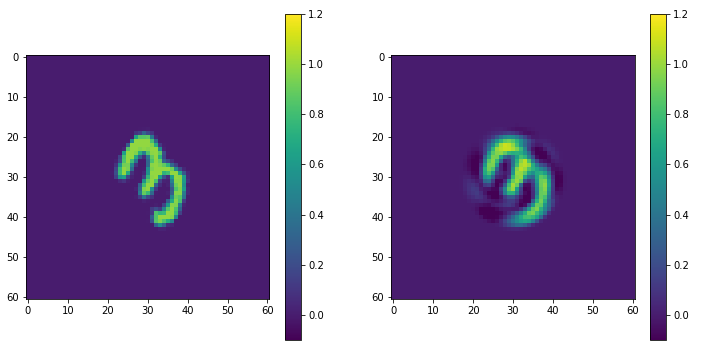
\includegraphics[scale=0.25]{rec_3_8.png}\\
\tiny{One random sample and its reconstruction using 8 PCs}
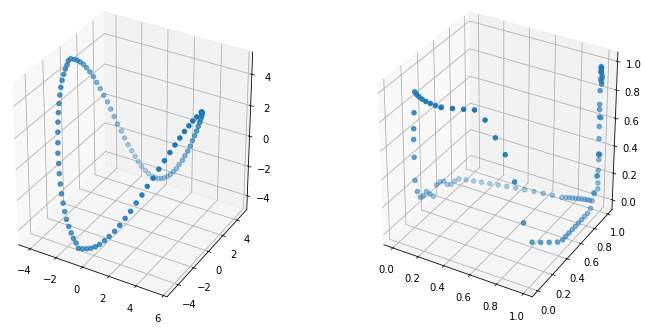
\includegraphics[scale=1.2]{scatterplot_pca.png}\\
\tiny{Scatterplot of the data in the first 3 PCs (left) or and a few well chosen pixels (right)}
\end{center}

\end{frame}


\begin{frame}{Examples in geosciences}
\textbf{Multi/Hyperspectral Images}

\begin{center}
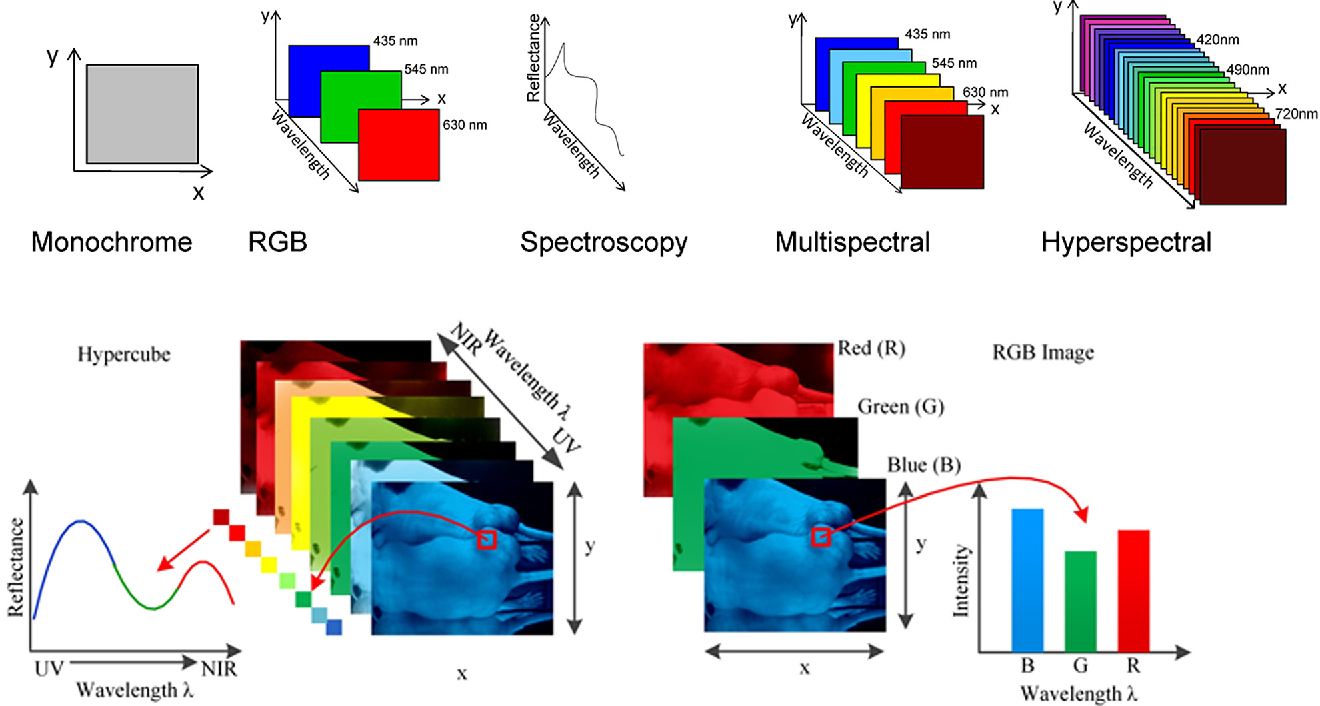
\includegraphics[scale = 0.25]{hyperspectral.png}
\end{center}

\begin{itemize}
\item images are matrices $\mathbf{X}\in\mathbb{R}^{D\times N}$, $D$ is the number of bands, $N$ is the number of pixels
\item Principal components are vectors $\mathbf{u}_{k} \in  \mathbb{R}^{D}$, and coefficients are vectors $\boldsymbol{a}_{k} \in \mathbb{R}^{N}$ (can be displayed as images)
\item $\mathbf{X} = \mathbf{U}\mathbf{A}$,  $\mathbf{U} \in \mathbb{R}^{D\times D}$, and $\mathbf{A} \in \mathbb{R}^{D\times N}$ 
\end{itemize}

\end{frame}


\begin{frame}{Examples in geosciences (cont'd)}

\textbf{Sea Surface Height/Temperature time series}

\begin{center}
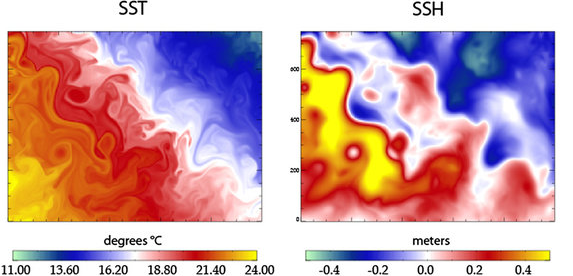
\includegraphics[scale = 1.6]{SST_SSH.png}
\end{center}

\begin{itemize}
\item data are matrices $\mathbf{X}\in\mathbb{R}^{D\times N}$, $N$ is the number time samples, $D$ is the number of pixels
\item Principal components are vectors $\mathbf{u}_{k} \in  \mathbb{R}^{D}$, and coefficients are vectors $\boldsymbol{a}_{k} \in \mathbb{R}^{N}$ (can be displayed as time series)
\item $\mathbf{X} = \mathbf{U}\mathbf{A}$,  $\mathbf{U} \in \mathbb{R}^{D\times D}$, and $\mathbf{A} \in \mathbb{R}^{D\times N}$ 
\end{itemize}

\end{frame}


\end{document}